\documentclass[12pt, a4paper, twoside, openright]{book}

\usepackage{vuwthesis} % sets up some local things, mostly the front page

\setlength{\intextsep}{12pt} % set space above and below in-line float
\setlength{\abovecaptionskip}{0pt} % set space between figure and caption.

\usepackage{amssymb, amsmath}
\usepackage{tikz}

\usepackage{etoolbox}
\newtoggle{compilealone}
\toggletrue{compilealone}

\title{Replicating John Philip 1972}
\author{Nat Lund}

\begin{document}

\chapter{Replicating John Philip 1972}\label{C:jrphilip}

The first known expression for an effective slip length appeared in 1972, in a paper in ZAMP by John R. Philip entitled ``Flows Satisfying Mixed No-Slip and No-Shear Conditions" \cite{Philip1972}.

In the paper, John R. Philip says that the limit of
\begin{equation}
W_{3} = \Im \left[  
 \alpha^{-1} \cos^{-1} 
 \left\{ \frac{\cos(\alpha \Theta)}{\cos \alpha} \right\} - \Theta
   \right]
\end{equation}
as $y\rightarrow \infty$ is
\begin{equation}
W_{3} = \alpha^{-1} \ln \sec \alpha
\end{equation}

Let us prove this forthwith.
\vspace*{1em}

$\Theta = x + iy$ is a complex number, $\alpha$ is real.  Trig identities for \emph{complex} cosine and exponential:
\begin{gather}
%\arccos z = - i \ln (z + \sqrt{z^{2} - 1}) \\
\cos z = \frac{e^{iz}+e^{-iz}}{2} \\
e^{i \theta} = \cos \theta + i \sin \theta 
\end{gather}

\clearpage
\section{Expand cosine term, dump negligible parts}

In Euler's formula $e^{i\theta} = cis(\theta)$, if $\theta$ is \emph{real}, then $e^{i \theta}$ traces out the unit circle in $\mathbb{C}$, with $\theta$ being the angle.

\begin{figure}[h]
\centering
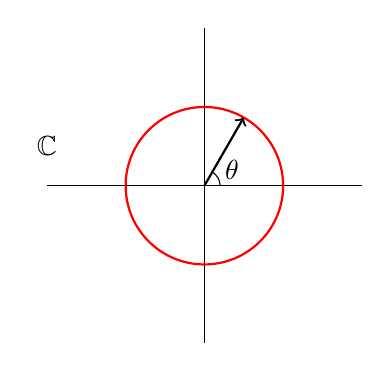
\begin{tikzpicture}
\draw (-2,0) -- ++ (4,0);
\draw (0,-2) -- ++(0,4);
\node at (-2,0.5) {$\mathbb{C}$};

\draw[thick, red] (0,0) circle (1cm);
\draw[thick,->] (0,0) -- ++(60:1);
\draw (0.2,0) arc  (0:60:2mm);
\node at (0.35,0.2) {$\theta$};

\end{tikzpicture}
\caption{Euler's formula $e^{i \theta}$ for real $\theta$ .}
\end{figure}


This gives insight into the $\cos z$ function.  If $z$ is real, then $\frac{1}{2} e^{iz}$ and $\frac{1}{2} e^{-iz}$ are two vectors of length $\frac{1}{2}$ that cycle in opposite directions, with $z$ being the angle. Then $\cos z$ is the sum of the two vectors, which always ends on the real line between -1 and 1, as shown in Figure (\ref{fig:cos}). 

\begin{figure}[h]
\centering
\begin{tikzpicture}
\draw (-4,0) -- ++ (8,0);
\draw (0,-2.5) -- ++(0,5);
\node at (-3,0.5) {$\mathbb{C}$};
\draw (4,0.1) -- ++(0,-0.2) node[below] {1};
\draw (-4,0.1) -- ++(0,-0.2) node[below] {-1};

\draw[thick, red, dashed] (0,0) circle (2cm);
\draw[thick, ->] (0,0) -- ++(45:2) -- ++(-45:2) node[below]{cos $z$};
\draw[thick, ->] (0,0) -- ++(45:2);
\node at (0.2,1)[right]{$\frac{1}{2} e^{iz}$};
\node at (2,1)[right]{$\frac{1}{2} e^{-iz}$};

\draw (0.3,0) arc  (0:45:3mm);
\node at (0.45,0.15) {$z$};

\draw[thick, dashed, ->] (0,0) -- ++(-45:2);
\draw (0.25,0) arc (0:-45:2.5mm);
\node at (0.5,-0.15) {$-z$};

\end{tikzpicture}
\caption{The complex cosine.} \label{fig:cos}
\end{figure}

With this insight, it is useful to rewrite $\cos z$ as:
\begin{equation}
\cos (x + iy) = \frac{ e^{i(x+iy)}+e^{-i(x+iy)} }{2} =
%\frac{ e^{ix - y} + e^{-ix + y} }{2} = 
e^{y} \frac{1}{2}e^{-ix} + e^{-y} \frac{1}{2} e^{ix}
\end{equation}

Then it is clear that $\cos (x + iy)$ is the sum of two rotating vectors in $\mathbb{C}$ with amplitudes $e^y$ and $e^{-y}$.  A consequence is that for large $y$, $e^y$ is \emph{very} large, while $e^{-y}$ is negligible, therefore $\cos (x + iy)$ is dominated by the vector $ e^{y} \frac{1}{2}e^{-ix} $.  See Figure (\ref{fig:coslargey}).

\begin{figure}[ht]
\centering
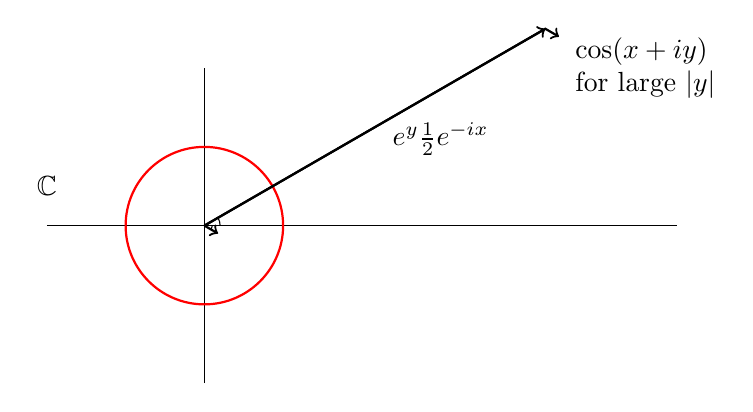
\begin{tikzpicture}
\draw (-2,0) -- ++ (8,0);
\draw (0,-2) -- ++(0,4);
\node at (-2,0.5) {$\mathbb{C}$};

\draw[thick, red] (0,0) circle (1cm);

\draw[thick,->] (0,0) -- ++(30:5) -- ++(-30:0.2);
\draw[thick,->] (0,0) -- ++(30:5);
\draw (0.2,0) arc  (0:30:2mm);
\draw[thick,->] (0,0) -- ++(-30:0.2);
\draw (0.1,0) arc (0:-30:1mm);

\node at (3,1.1) {$e^{y} \frac{1}{2}e^{-ix}$};
{
\renewcommand{\baselinestretch}{1.00}
\node at (5.6,2)[align=left] {$\cos (x+iy)$\\ for large $|y|$};
}
\end{tikzpicture}
\caption{Complex cosine at large $|y|$.} \label{fig:coslargey}
\end{figure}

\begin{equation}
\text{Therefore} \quad \cos (x + iy) \to  \frac{e^{y} e^{-ix}}{2}
\quad \text{as} \quad y \to \infty
\end{equation}

\begin{equation}
\cos z \to \frac{1}{2} e^{-iz} \quad \text{as} \quad y \to \infty
\end{equation}


\section{Inverse Cosine at Large $y$}

As $y \to \infty$:
\begin{equation}
w = \cos z \to \frac{1}{2} e^{-iz}
\end{equation}
Solve $w = \cos z$ for $z$ to get:
\begin{equation*}
\arccos w = z
\end{equation*}
Likewise solve $w = \frac{1}{2} e^{-iz}$ for $z$:
\begin{gather*}
w = \frac{1}{2} e^{-iz} \\
2 w = e^{-iz} \\
\ln (2w) = -iz \\
%\text{Multiply both sides by }i \\
i \ln (2w) = -i^2 z \\
%\text{Now, } -i^2 = 1, \text{  so} \\
i \ln (2w) = z
\end{gather*}
Equate the two expressions to obtain the inverse cosine in terms of a logarithm:
\begin{equation}
\arccos z = i \ln(2z)
\end{equation}

\section{Put into J.\ R.\ Philip's Expression}

\begin{equation}
W_{3} = \Im \left[  
 \alpha^{-1} \cos^{-1} 
 \left\{ \frac{\cos(\alpha \Theta)}{\cos \alpha} \right\} - \Theta
   \right]
\end{equation}

As $y \to \infty$, the cosine expression may be substituted:

\begin{equation}
W_{3} = \Im \left[  
 \alpha^{-1} \cos^{-1} 
 \left\{ \frac{\frac{1}{2} e^{-i \alpha \Theta}}{\cos \alpha} \right\} - \Theta
   \right]
\end{equation}

And the inverse cosine expression may also be substituted:

\begin{equation}
W_{3} = \Im \left[  
 i \alpha^{-1} \ln 
 \left\{ 2 \frac{\frac{1}{2} e^{-i \alpha \Theta}}{\cos \alpha} \right\} - \Theta
   \right]
\end{equation}

\begin{equation}
W_{3} = \Im \left[  
 i \alpha^{-1} \ln 
 \left\{ e^{-i \alpha \Theta} \frac{1 }{\cos \alpha} \right\} - \Theta
   \right]
\end{equation}

Recall that $\ln ab = \ln a + \ln b$.

\begin{equation}
W_{3} = \Im \left[  
 i \alpha^{-1} \ln 
 \left\{ e^{-i \alpha \Theta}  \right\}
+
i \alpha^{-1} \ln 
 \left\{ \frac{1 }{\cos \alpha} \right\} 
  - \Theta
   \right]
\end{equation}

Invoke definition of logarithm: $\ln e^z = z$.

\begin{equation}
W_{3} = \Im \left[  
 i \alpha^{-1} 
 \left\{ -i \alpha \Theta  \right\}
+
i \alpha^{-1} \ln 
 \left\{ \frac{1 }{\cos \alpha} \right\} 
  - \Theta
   \right]
\end{equation}

%\begin{equation}
%W_{3} = \Im \left[  
% -i^2 \alpha^{-1} \alpha \Theta
%+
%i \alpha^{-1} \ln 
% \left\{ \frac{1 }{\cos \alpha} \right\} 
%  - \Theta
%   \right]
%\end{equation}

\begin{equation}
W_{3} = \Im \left[  
\Theta
+
i \alpha^{-1} \ln 
 \left\{ \frac{1 }{\cos \alpha} \right\} 
  - \Theta
   \right]
\end{equation}

\begin{equation}
W_{3} = \Im \left[  
i \alpha^{-1} \ln 
 \left\{ \frac{1 }{\cos \alpha} \right\} 
   \right]
\end{equation}

%\begin{equation}
%W_{3} =
%\alpha^{-1} \ln 
% \left\{ \frac{1 }{\cos \alpha} \right\} 
%\end{equation}

\begin{equation}
W_{3} =
\alpha^{-1} \ln \sec \alpha
\end{equation}

We have demonstrated that which we set out to prove.
%As required.

\iftoggle{compilealone}
    {
    \bibliography{Lund_Thesis.bib}
    \bibliographystyle{plain}
    }

\end{document}





%The complex cosine term in J. R. Philip's expression is:
%\begin{equation}
%\left\{ \frac{\cos(\alpha \Theta)}{\cos \alpha} \right\} = 
%\left\{ \frac{\cos(\alpha(x + iy)}{\cos \alpha} \right\} =
%\left\{ \frac{\cos(\alpha x + i \alpha y)}{\cos \alpha} \right\}
%\end{equation}
%For any fixed real $\alpha$, as $y \to \infty$,
%\begin{equation}
%\left\{ \frac{\cos(\alpha x + i \alpha y)}{\cos \alpha} \right\} \to
%\left\{ \frac{ e^{\alpha y} e^{-i\alpha x} }{2 \cos \alpha} \right\}
%\end{equation}
%The magnitude of this complex number tends to infinity as $y \to \infty$.
%
%\end{document}
